\section{REPL Commands}
\label{sec:commands}

To separate the implementation of user operations into logical units, each user
operation is encapsulated within a class implementing the
\texttt{``IReplCommand''} interface. See \cref{fig:uml-commands} for the design
of the \texttt{commands} package. After acquiring an invoker instance, the
frontend has two commands available by default:

\begin{description}
  \item [:load] \texttt{LanguageCommand}, loads a language from a file path;
  \item [:help] \texttt{HelpCommand}, prints descriptions of all available commands.
\end{description}

\begin{figure}[h]
  \centering
  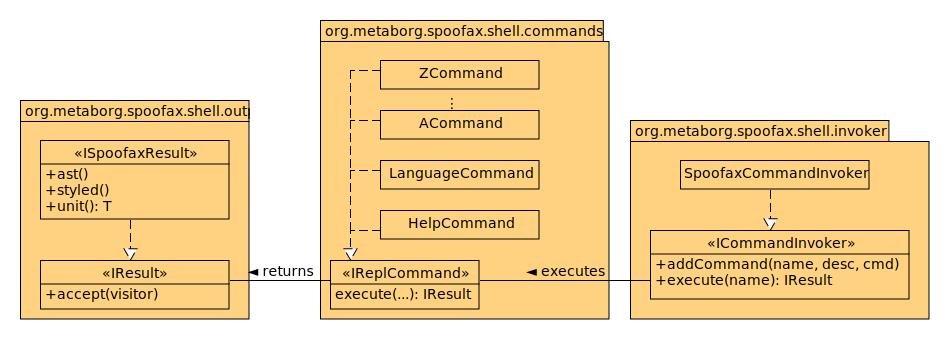
\includegraphics[width=\textwidth]{uml-commands}
  \caption{UML of the various commands frontends can execute and the
           corresponding result interfaces.}
  \label{fig:uml-commands}
\end{figure}

Frontends can define additional commands by implementing the
\texttt{``IReplCommand''} interface. These commands can then be made available
to the invoker by either binding them in the default map of available commands
via a Guice module or by adding an entry to the invoker at runtime using the
\texttt{``addCommand''} method.

As explained in the introduction of this chapter, there are only a few
commands that work across all languages, since every language can define its
own transformations or evaluation strategy. Therefore, the
\texttt{LanguageCommand} tries to determine several properties of the loaded
language and adjusts the set of loaded commands accordingly.

By splitting operations in small logical units the design ensures command
classes adhere to the Single Responsibility principle, which makes all REPL
commands less complex and therefore easier to maintain. The logical units that
make up the commands also ensure a flexible design that can be modified
as the Spoofax architecture develops further on.

% FIXME: Belongs in implementation chapter probably.
%The ``LanguageCommand'' tries to load a language using the Spoofax services.
%When Spoofax succeeds in loading the language, the parameters set in the
%language facets (specifically the AnalysisFacet and the ShellFacet) are used to
%create a set of commands that should be available for this specific language
%through the ``CommandBuilder'' class. The resulting set of commands consists of
%the following commands:
%
%\begin{description}
%  \item [:parse] Parses the given arguments and returns a corresponding AST.
%  \item [:analyze] Performs static analysis on the input. Not available in all languages.
%  \item [:evaluate] Evaluates the given input and returns the execution result.
%\end{description}
%
%Furthermore a command is created for each transform goal specified through the
%Spoofax MenuService. The transform commands are identified by their name as
%specified in ESV. The process of building commands will be explained in more
%depth in \cref{sec:function-comp}. By making all these commands

%%% Local Variables:
%%% TeX-master: "../main"
%%% End:
